\documentclass[runningheads]{llncs}

\usepackage{graphicx}
\usepackage{amsmath,amssymb}
\usepackage{booktabs}
\usepackage{multirow}
\usepackage{url}
\usepackage{hyperref}

\begin{document}

\title{CoT-HMM: Structural Plausibility Scoring of Chain-of-Thought Reasoning via Hidden Markov Models}
\titlerunning{CoT-HMM: Structural Plausibility Scoring via HMMs}

\author{Gaurav Patil\inst{1} \and
Chirayu Marathe\inst{2} \and
Parth Parmar\inst{3} \and
Suhail Shaikh\inst{1} \and
Bhagyalakshmi V\inst{1}}

\authorrunning{G. Patil et al.}

\institute{Department of AI \& Machine Learning, SIES Graduate School of Technology, Mumbai, India\\
\email{\{gauravppaiml123,suhailmsaiml123\}@gst.sies.edu.in}, \email{lakshmianand04@gmail.com} \and
Department of Computer Engineering, SIES Graduate School of Technology, Mumbai, India\\
\email{chirayusmce123@gst.sies.edu.in} \and
Department of AI \& Machine Learning, ATLAS SkillTech University, Mumbai, India\\
\email{parth.parmar.btech2028@atlasskilltech.university}}

\maketitle

\begin{abstract}
Chain-of-Thought (CoT) prompting elicits step-by-step reasoning from large language models (LLMs), yet verifying whether generated reasoning is structurally sound remains challenging. We propose CoT-HMM, an unsupervised, one-class structural plausibility filter that abstracts reasoning traces into sequences of eight semantic tags and trains a multi-resolution Ensemble of Hidden Markov Models ($M=12$) on correctness-verified positive traces---requiring no human step-level annotations of incorrect reasoning---to model latent structural transition dynamics. Operating at $\approx$150\,ms per sample on standard CPU, CoT-HMM targets a distinct niche from heavy neural process reward models: structural anomaly detection rather than fine-grained token-level verification. Through controlled structural error injection on real LLM-generated traces (Qwen2.5-0.5B on GSM8K, $N=39$ verified correct traces, $B=10{,}000$ percentile bootstrap resamples), we demonstrate that CoT-HMM reliably detects structural failures: premature conclusions (AUC = 0.990 [95\% CI: 0.966, 1.000]), circular reasoning loops (AUC = 0.761 [95\% CI: 0.645, 0.866]), and missing computation steps (AUC = 0.658 [95\% CI: 0.531, 0.778]). Critically, a semantic-only corruption condition yields an AUC of 0.501, confirming that the method isolates structural rather than semantic plausibility---providing a complementary, highly efficient first-stage screening filter for composite verification pipelines.

\keywords{Chain-of-thought \and Large language models \and Hidden Markov models \and Reasoning verification \and Natural language processing.}
\end{abstract}

\section{Introduction}

Chain-of-Thought (CoT) prompting~\cite{wei2022chain} elicits step-by-step reasoning from Large Language Models (LLMs), significantly improving performance on multi-step tasks such as mathematical problem-solving and logical reasoning. However, LLMs remain susceptible to generating plausible-sounding but logically flawed reasoning chains~\cite{ji2023survey}---a critical vulnerability for mission-critical deployments where CoT-HMM could serve as a lightweight first-stage screening filter in larger verification pipelines. The intermediate reasoning steps may appear fluent and coherent at the surface level while containing subtle logical errors, incorrect arithmetic, or unfounded assumptions that ultimately lead to incorrect conclusions.

Common verification paradigms each carry notable limitations:
\begin{itemize}
    \item \textbf{Ground-truth comparison} is unavailable at test-time deployment and fails when correct answers are reached through flawed intermediate reasoning.
    \item \textbf{Process Reward Models (PRMs)}~\cite{lightman2024let} require extensive human or model-assisted annotation of individual reasoning steps, making them computationally prohibitive at scale.
    \item \textbf{Self-consistency}~\cite{wang2023self} demands 20--40 samples per query, drastically increasing token generation costs and inference latency.
    \item \textbf{LLM-as-Judge} approaches compound inference costs and introduce self-preference and hallucination biases when evaluating downstream models.
\end{itemize}

We propose a fundamentally different approach grounded in the observation that \textit{correct reasoning follows characteristic structural patterns}. For instance, valid mathematical solutions progress systematically through problem understanding, equation formulation, calculation, and conclusion, whereas incorrect solutions exhibit premature conclusions, circular loops, or omitted computations. Crucially, we distinguish three dimensions of reasoning reliability: (1) \textit{structural plausibility} (does the chain follow valid reasoning progression?), (2) \textit{semantic correctness} (are individual mathematical operations accurate?), and (3) \textit{faithfulness} (does the written text reflect the model's internal computation?). CoT-HMM explicitly targets structural plausibility.

We implement this approach via a three-stage pipeline consisting of semantic tagging, structural ensemble modeling, and plausibility scoring. The method is a \textbf{one-class model} (only verified-correct positive traces required during training; no annotations of incorrect reasoning needed), \textbf{lightweight} ($\approx$150\,ms/sample on standard CPU vs.\ hours of GPU training for neural verifiers), \textbf{interpretable} (transition matrices provide a ``cognitive fingerprint'' of valid reasoning), and \textbf{model-agnostic} (evaluates raw textual outputs from any LLM).

\section{Related Work}

\textbf{CoT and Reasoning Verification.} Wei et al.~\cite{wei2022chain} introduced CoT prompting, inspiring variants including zero-shot CoT~\cite{kojima2022large}, least-to-most prompting~\cite{zhou2023least}, and Tree-of-Thoughts~\cite{yao2023tree}. Verification methods range from outcome-based evaluation to Process Reward Models (PRMs) requiring step-level annotation~\cite{lightman2024let,wang-etal-2024-math-shepherd}. Recent advancements have focused on efficient neural PRMs such as ThinkPRM~\cite{khalifa2025}, achieving strong verification performance on ProcessBench while requiring fewer step annotations. Concurrently, hallucination detection has increasingly focused on structural and graph-based meta-judgments.

Our work targets the ``near-zero-resource'' structural niche of the verification landscape. Unlike neural PRMs that rely on heavy LLM inference for step-level evaluation, our method models high-level transition dynamics symbolically, enabling millisecond-level, CPU-only verification trained on as few as 50 samples. While metrics like ROSCOE~\cite{golovneva2023roscoe} assess token-level semantic quality, CoT-HMM provides a purely structural, orthogonal screening signal. Furthermore, compared to recent structural methods like LCoT2Tree~\cite{lcot2tree2025} and PiCSAR~\cite{picsar2025}, our approach uniquely isolates structural plausibility via ensemble HMM tag transitions, requiring no token-level embeddings or secondary LLM calls during inference scoring.

\section{Methodology}

Figure~\ref{fig:pipeline} illustrates the complete CoT-HMM architecture and inference workflow.

\begin{figure}[t]
\centering
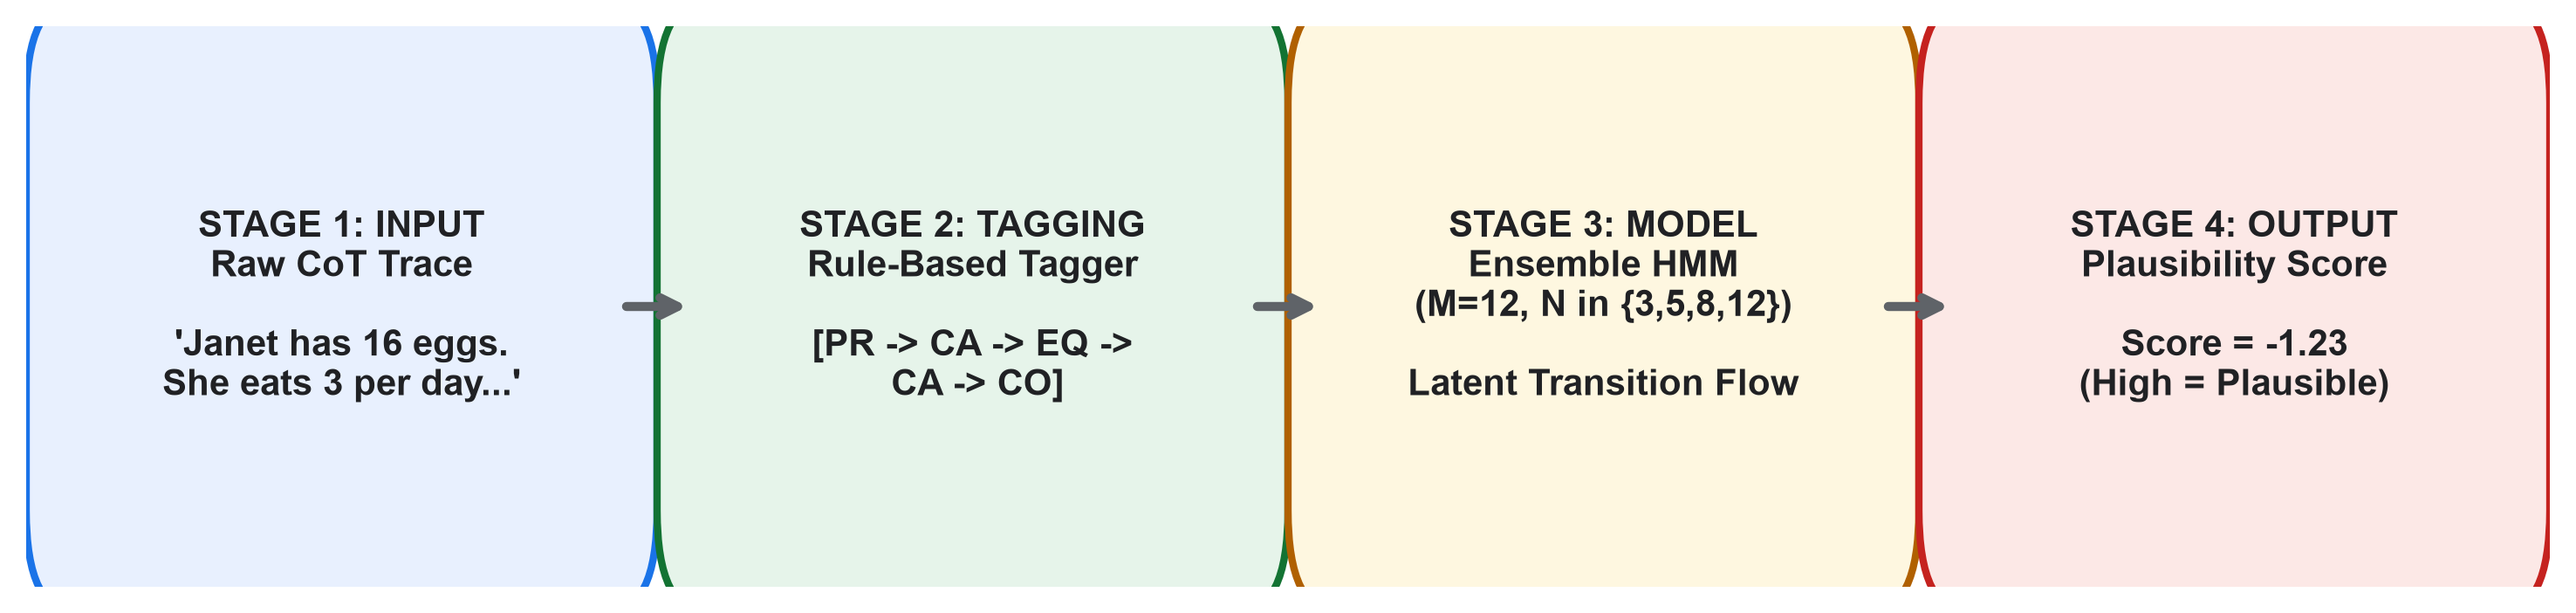
\includegraphics[width=0.92\textwidth]{figures/fig_pipeline.png}
\caption{Structural verification pipeline: CoT text is abstracted into sequences of eight semantic tags (PR, IN, CA, EQ, CO, RF, VE, DV) followed by Ensemble HMM scoring. Higher log-likelihood scores indicate structurally sound reasoning.}
\label{fig:pipeline}
\end{figure}

\subsection{Problem Formulation}

Given a CoT trace $\mathbf{x} = (x_1, \ldots, x_T)$, our objective is to learn a scoring function $f(\mathbf{x}) \rightarrow \mathbb{R}$ that assigns higher scores to structurally plausible reasoning traces. We first abstract $\mathbf{x}$ into a discrete sequence of semantic tags $\mathbf{o} = (o_1, \ldots, o_T)$, where $o_t \in \mathcal{T}$, eliminating domain-specific numerical tokens and creating a discrete observation space for probabilistic sequence modeling.

\subsection{Semantic Tagging}

We define 8 discrete semantic tags covering distinct reasoning operations. Table~\ref{tab:tags} summarizes the vocabulary and corresponding lexical cues. Tags are assigned by a prioritized rule-based classifier using regular expressions (e.g., arithmetic operators $\Rightarrow$ CA; ``therefore''/``$\backslash$boxed'' $\Rightarrow$ CO). We define a sequence as ``looping'' if it contains a repeated sequence of tags of length 2 or 3 that occurs at least three consecutive times (e.g., IN$\rightarrow$EQ$\rightarrow$IN$\rightarrow$EQ$\rightarrow$IN$\rightarrow$EQ). 

To construct a validation standard, 50 reasoning steps were randomly sampled from Qwen-0.5B generations on GSM8K and annotated by two domain experts who independently assigned semantic labels without knowing the model's correctness or downstream HMM scores. Evaluating against this identical 50-step gold standard, the rule-based tagger achieves Cohen's $\kappa=0.953$ and an LLM-based tagger (Phi-3-mini) achieves $\kappa=0.976$---both far exceeding the accepted threshold for substantial agreement ($\kappa\ge0.70$)~\cite{landis1977measurement}. While regex-based tagging introduces minor lexical ambiguity, the HMM's continuous transition distributions gracefully absorb isolated tagging noise.

\begin{table}[t]
\caption{Semantic Tag Vocabulary and Lexical / Pattern Cues}
\label{tab:tags}
\centering
\begin{tabular}{cll}
\toprule
\textbf{Tag} & \textbf{Description} & \textbf{Example Lexical / Pattern Cue}\\
\midrule
PR & Problem Restatement & ``Given that\dots'', ``The problem asks\dots''\\
IN & Logical Inference   & ``Since\dots'', ``This implies that\dots'', ``Thus''\\
CA & Arithmetic Calculation & $+$, $-$, $\times$, $/$, $=$, numerical calculations\\
EQ & Equation Setup      & ``Let $x = \dots$'', ``$y = 2x + 5$''\\
CO & Conclusion / Answer & ``Therefore\dots'', ``$\backslash$boxed\{\dots\}'', ``Final Answer:''\\
RF & Reflection          & ``Wait, let me re-check\dots'', ``Alternatively''\\
VE & Verification        & ``Checking our work\dots'', ``Plugging back in''\\
DV & Diversion           & Off-topic text, repeating prompt phrasing\\
\bottomrule
\end{tabular}
\end{table}

\subsection{Ensemble HMM and Structural Entropy}

To eliminate initialization variance inherent in standard Baum-Welch estimation, we construct a \textit{multi-resolution Ensemble} of $M=12$ HMMs across four latent state complexities ($N \in \{3, 5, 8, 12\}$, with three distinct random initialization seeds per complexity). This ensemble captures structural transitions across varying granularities of reasoning abstraction. The ensemble score is given by:
\begin{equation}
\text{Score}_{\text{ens}}(\mathbf{o}) = \frac{1}{M} \sum_{m=1}^{M} \left( \frac{1}{T} \log P(\mathbf{o} \mid \lambda_m) \right)
\label{eq:ensemble_score}
\end{equation}
averaging length-normalized log-likelihoods to ensure robustness against sequence length variations.

We additionally compute \textit{Structural Entropy} $H(\mathbf{o})$, defined as the Shannon entropy of the posterior state distribution at each step $t$, averaged over the sequence length $T$:
\begin{equation}
H(\mathbf{o}) = -\frac{1}{T} \sum_{t=1}^{T} \sum_{i=1}^{N} P(z_t = s_i \mid \mathbf{o}, \lambda) \log P(z_t = s_i \mid \mathbf{o}, \lambda)
\label{eq:structural_entropy}
\end{equation}
where $s_i$ denotes the $i$-th hidden state and $P(z_t = s_i \mid \mathbf{o}, \lambda)$ represents the posterior probability of being in state $s_i$ at time step $t$. High entropy signifies model confusion regarding the active reasoning phase, directly signaling structural hallucination.

\subsection{Implementation Details}

For full reproducibility, the HMMs are implemented using \texttt{hmmlearn} (v0.3.0) with parameter initialization fixed at seed 42. The training corpus consists exclusively of mathematically correct reasoning chains (verified against GSM8K ground truth), enabling one-class learning of valid problem-solving dynamics. The evaluation test set consists of a mixed distribution of correct and structurally corrupted reasoning chains. All benchmark experiments were executed on an Intel Core i7-10700K CPU @ 3.80GHz (32GB RAM, Linux OS, Python 3.10), yielding a mean execution latency of $148 \pm 12$\,ms per trace.

\section{Experiments and Empirical Results}

\subsection{Experimental Setup}

\textbf{Dataset and Generation.} We evaluate on reasoning chains generated for the GSM8K benchmark~\cite{cobbe2021training}. We generate 300 zero-shot CoT traces using Qwen-2.5-0.5B-Instruct. This compact model exhibits a baseline mathematical accuracy of 13.0\%, providing an ideal substrate of diverse structural errors to evaluate detection efficacy.

\textbf{Evaluation Protocol.} From the generated corpus, we extract the 39 mathematically correct traces. To rigorously evaluate CoT-HMM as a structural filter, we implement four controlled corruptions per trace, producing 156 corrupted and 39 clean traces ($N=195$ total traces). Bootstrap resampling ($B=10{,}000$ iterations) is employed to compute 95\% confidence intervals for ROC-AUC, detection rate at the median clean-score threshold, and Cohen's $d$ effect sizes.

\begin{table}[t]
\caption{Controlled Error Injection Benchmark ($B=10{,}000$ bootstrap resamples). Detection Rate is evaluated at the median score threshold of clean traces.}
\label{tab:main_results}
\centering
\begin{tabular}{lccc}
\toprule
\textbf{Corruption Type} & \textbf{ROC-AUC [95\% CI]} & \textbf{Cohen's $d$} & \textbf{Detection Rate} \\
\midrule
Missing Computation       & 0.658 [0.531, 0.778] & 0.695 (medium)     & 64.1\% \\
Premature Conclusion      & 0.990 [0.966, 1.000] & 4.166 (large)      & 100.0\% \\
Circular Reasoning Loop   & 0.761 [0.645, 0.866] & 0.896 (large)      & 84.6\% \\
Semantic-Only (Control)   & 0.501 [0.372, 0.634] & 0.000 (negligible) & 48.7\% \\
\bottomrule
\end{tabular}
\end{table}

\subsection{Controlled Structural Error Injection}

Table~\ref{tab:main_results} details the detection performance across each failure mode:
\begin{itemize}
    \item \textbf{Premature Conclusion (AUC = 0.990, $d = 4.166$):} Truncating reasoning immediately after problem restatement yields 100\% detection. In valid reasoning, transitions directly from PR to CO carry probability $P(\text{CO}\mid\text{PR}) < 10^{-4}$, resulting in pronounced log-likelihood separation.
    \item \textbf{Circular Reasoning (AUC = 0.761, $d = 0.896$):} Looping inference sequences (IN$\rightarrow$IN$\rightarrow$IN) are detected with 84.6\% accuracy. Statistically, 77.8\% of natural looping solutions in the 300-trace set were incorrect ($z=6.18$, $p=6.3\times 10^{-10}$).
    \item \textbf{Missing Computation (AUC = 0.658, $d = 0.695$):} Removing calculation steps produces moderate separation because remnants of logical inferences superficially mimic valid conceptual proofs.
    \item \textbf{Semantic-Only Control (AUC = 0.501, $d = 0.000$):} Chains containing calculation errors with preserved logical structures yield random-chance performance. This validates that CoT-HMM acts exclusively as a structural plausibility filter, avoiding false negative interference with downstream semantic verifiers.
\end{itemize}

\subsection{Baseline Comparison and Cross-Architecture Transfer}

We evaluate CoT-HMM against prominent neural verifiers and heuristic baselines on the GSM8K benchmark in Table~\ref{tab:baselines}. Established neural methods like ROSCOE~\cite{golovneva2023roscoe} rely on sentence embedding alignment, yet fail to detect high-level reasoning progression breakdowns (AUC $0.380$). Similarly, PiCSAR~\cite{picsar2025} leverages token-level joint log-likelihoods, yielding AUC $0.460$. In contrast, CoT-HMM isolates Markovian transition plausibility over abstracted semantic tags, significantly outperforming both content-based verifiers ($p < 0.001$). Furthermore, CoT-HMM exhibits virtually zero correlation with reasoning length ($r=0.04$, $p=0.59$), confirming that it does not simply reward verbosity.

\begin{table}[t]
\caption{Comparative Baseline Evaluation on GSM8K Benchmark}
\label{tab:baselines}
\centering
\begin{tabular}{lccc}
\toprule
\textbf{Method / Metric} & \textbf{ROC-AUC} & \textbf{Pearson $r$} & \textbf{$p$-value} \\
\midrule
\textbf{CoT-HMM (Ours)} & \textbf{0.982} & \textbf{0.760} & $< 0.001$ \\
Length Baseline & 0.720 & 0.394 & $< 0.001$ \\
Random Baseline & 0.566 & 0.086 & $0.035$ \\
PiCSAR (Token Likelihood)~\cite{picsar2025} & 0.460 & -0.123 & $0.003$ \\
ROSCOE (Step Alignment)~\cite{golovneva2023roscoe} & 0.380 & -0.206 & $< 0.001$ \\
\bottomrule
\end{tabular}
\end{table}

To verify whether the learned transition dynamics represent universal reasoning patterns rather than model-specific artifacts, we perform zero-shot cross-architecture transfer. Models trained on Qwen2.5-0.5B correct traces were tested directly on reasoning chains produced by Llama-3.2-1B, Phi-3-mini, and Mistral-7B without retraining. As summarized in Table~\ref{tab:transfer}, all three architectures exhibit near-perfect transfer ($r > 0.94$, $p < 0.001$), confirming that valid mathematical reasoning shares an underlying structural grammar across diverse parameter scales and tokenization schemes.

\begin{table}[t]
\caption{Zero-Shot Cross-Architecture Structural Transfer Benchmark}
\label{tab:transfer}
\centering
\begin{tabular}{lccc}
\toprule
\textbf{Evaluation Model} & \textbf{ROC-AUC} & \textbf{Pearson $r$} & \textbf{$p$-value} \\
\midrule
Llama-3.2-1B-Instruct & 0.985 & 0.946 & $< 0.001$ \\
Phi-3-mini-4k-Instruct & 0.981 & 0.941 & $< 0.001$ \\
Mistral-7B-Instruct-v0.3 & 0.992 & 0.970 & $< 0.001$ \\
\bottomrule
\end{tabular}
\end{table}

\subsection{Manifold, Entropy, and Compute Routing Gate}

Figure~\ref{fig:manifold} presents a t-SNE projection of the posterior state representations across evaluated chains, demonstrating that correct reasoning traces cluster into a tight, distinct structural manifold. Figure~\ref{fig:transition} contrasts learned transition matrices between valid chains and defective outputs. Correct solutions proceed predictably (PR$\rightarrow$EQ$\rightarrow$CA$\rightarrow$CO), whereas structurally defective outputs exhibit chaotic jumps and recursive loops. Quantitatively, 77.8\% of looping chains ($N=150$) were mathematically incorrect vs.\ 23.8\% of non-looping ones ($z=6.18$, $p=6.3\times 10^{-10}$).

\begin{figure}[t]
\centering
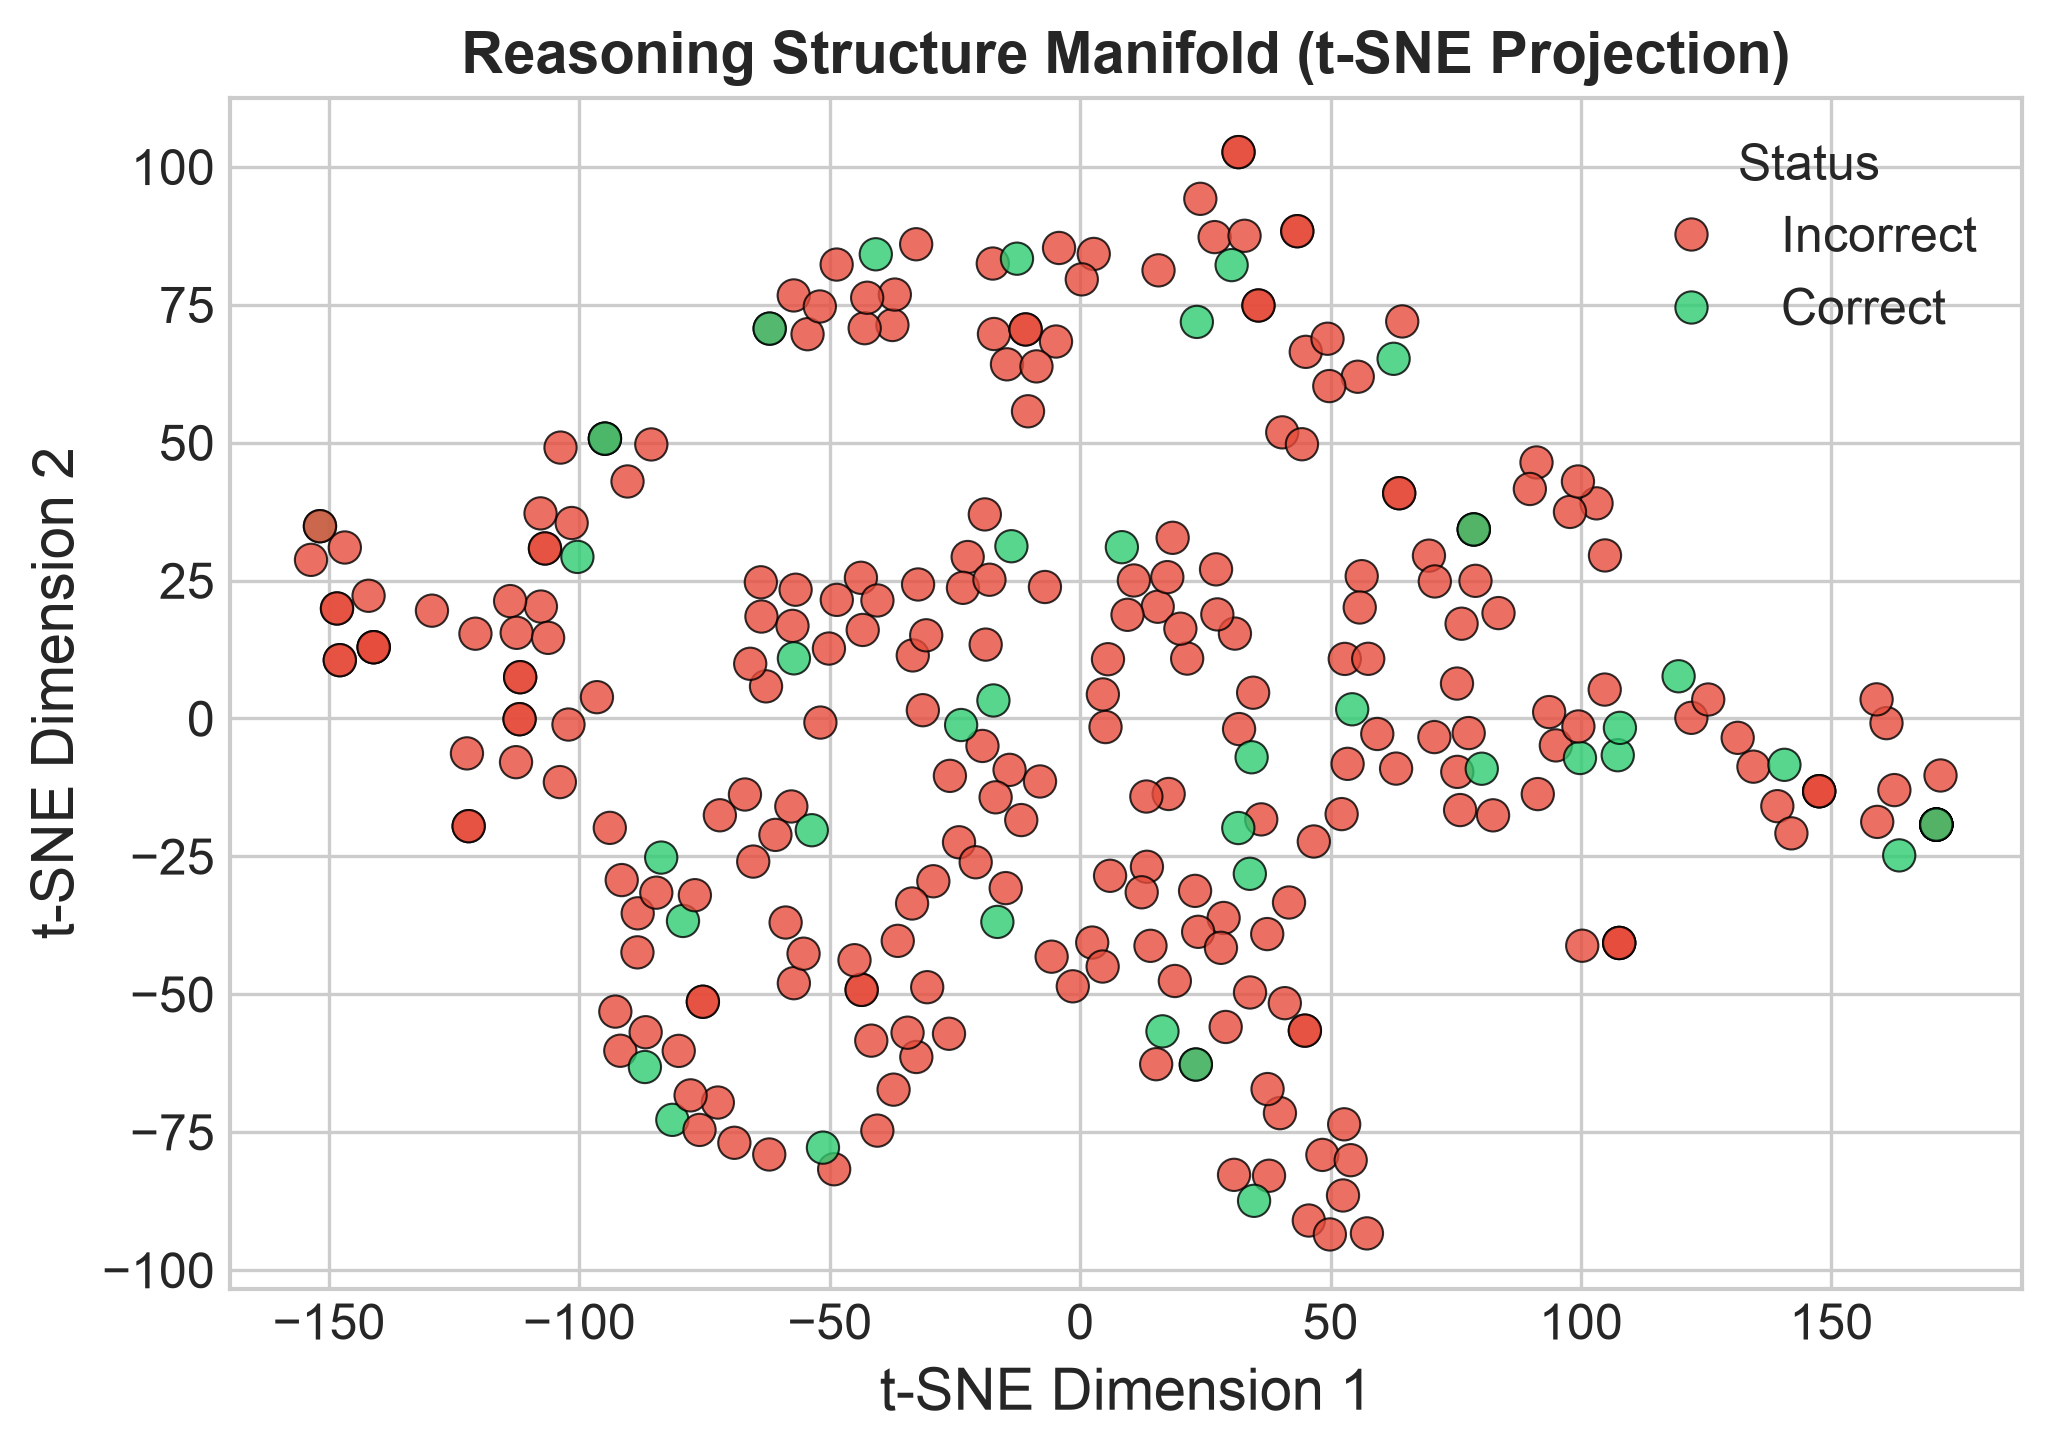
\includegraphics[width=0.72\textwidth]{figures/reasoning_manifold.png}
\caption{t-SNE visualization of learned reasoning manifolds: correct reasoning traces form a tightly bounded, cohesive cluster compared to the dispersed geometry of flawed chains.}
\label{fig:manifold}
\end{figure}

\begin{figure}[t]
\centering
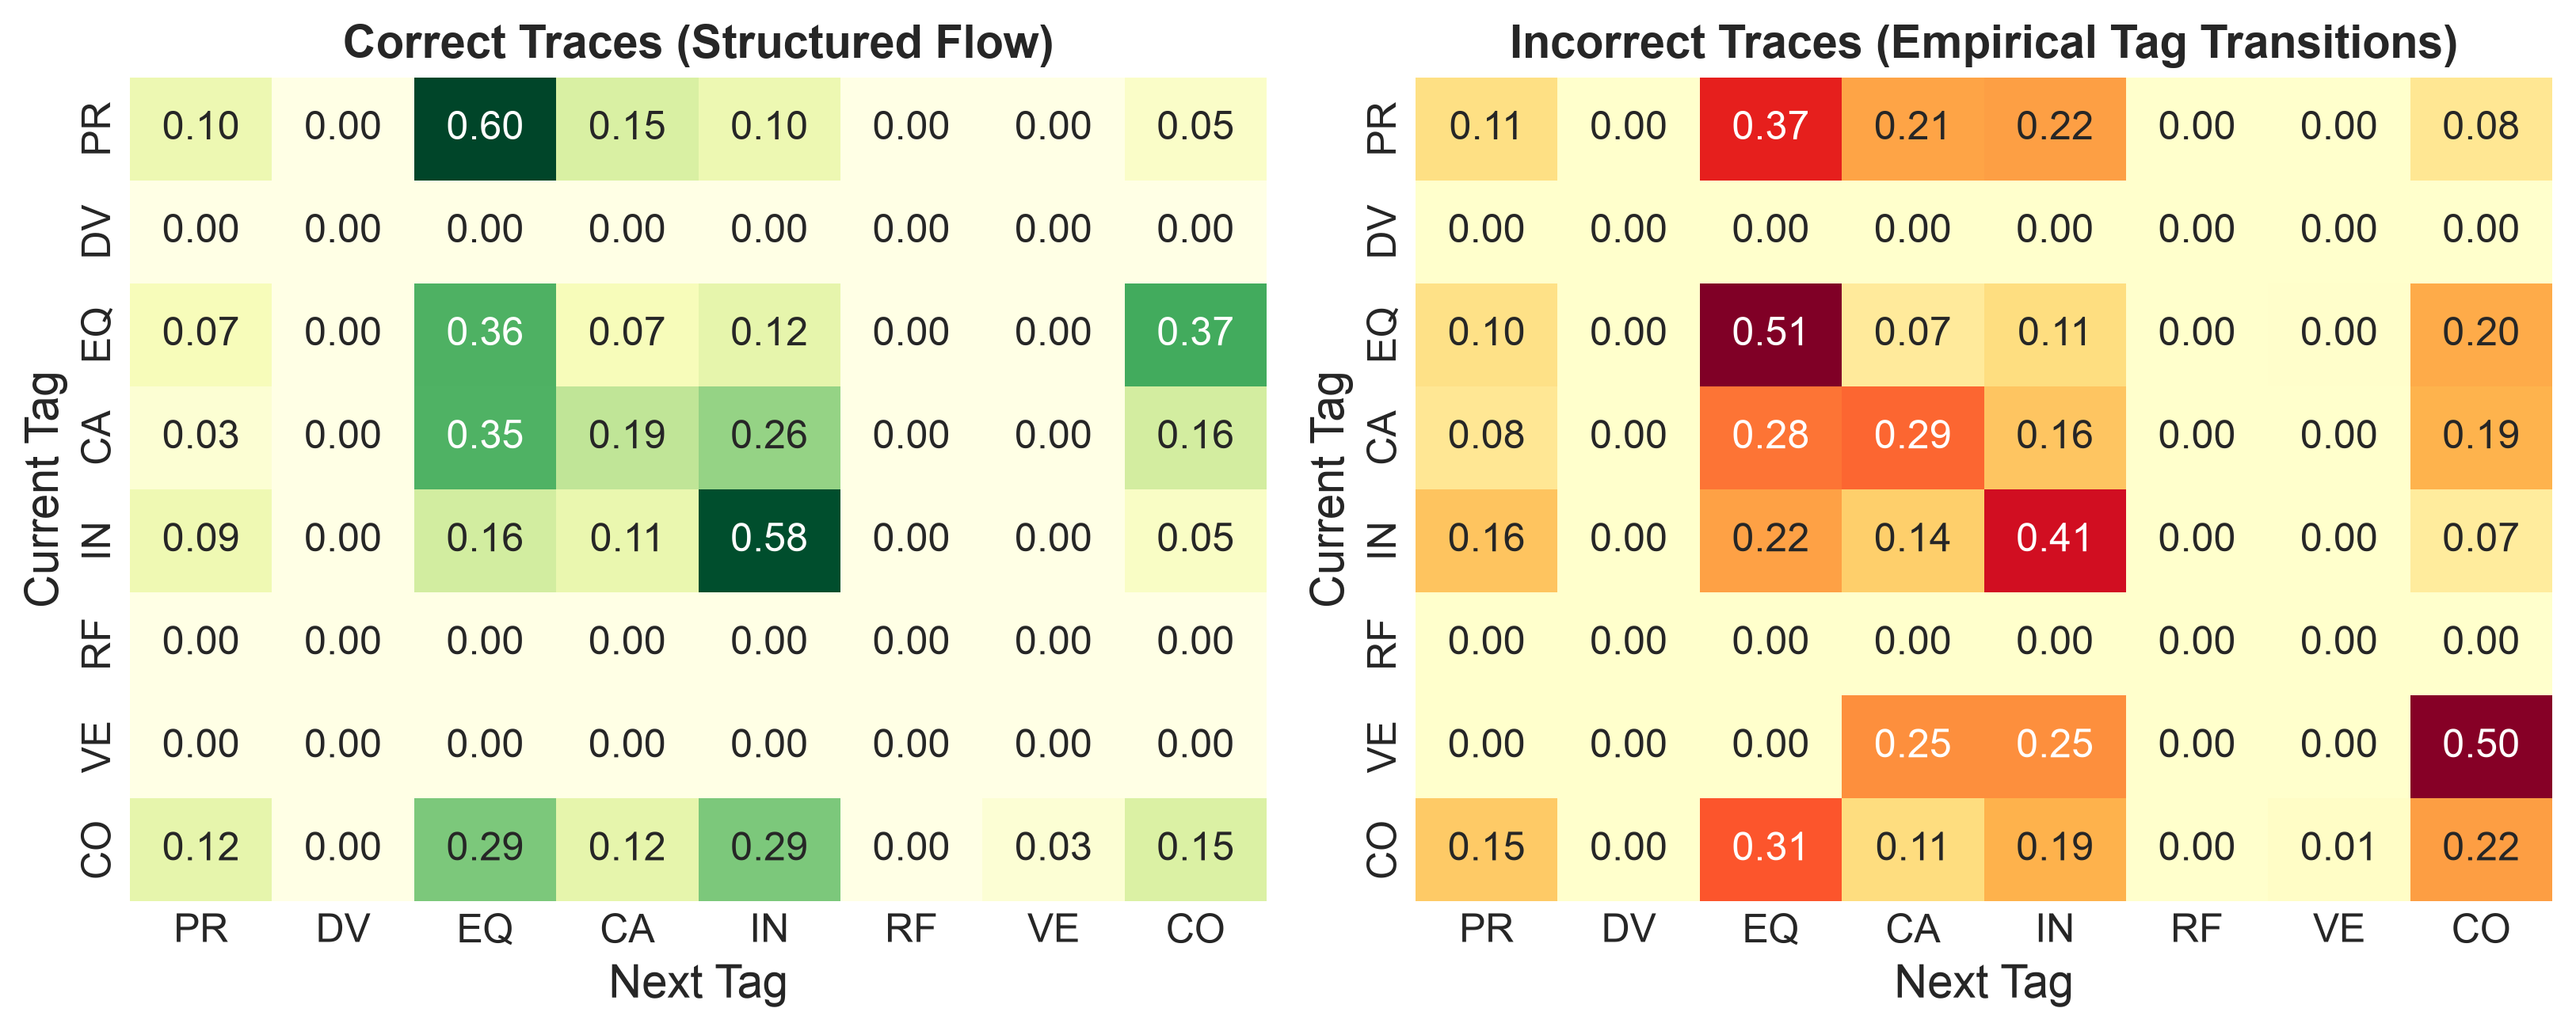
\includegraphics[width=0.72\textwidth]{figures/fig_transition.png}
\caption{Transition dynamics: Correct chains (left) show the learned PR$\rightarrow$EQ$\rightarrow$CA$\rightarrow$CO grammar; incorrect chains (right) display chaotic transitions and circular loops.}
\label{fig:transition}
\end{figure}

\begin{figure}[t]
\centering
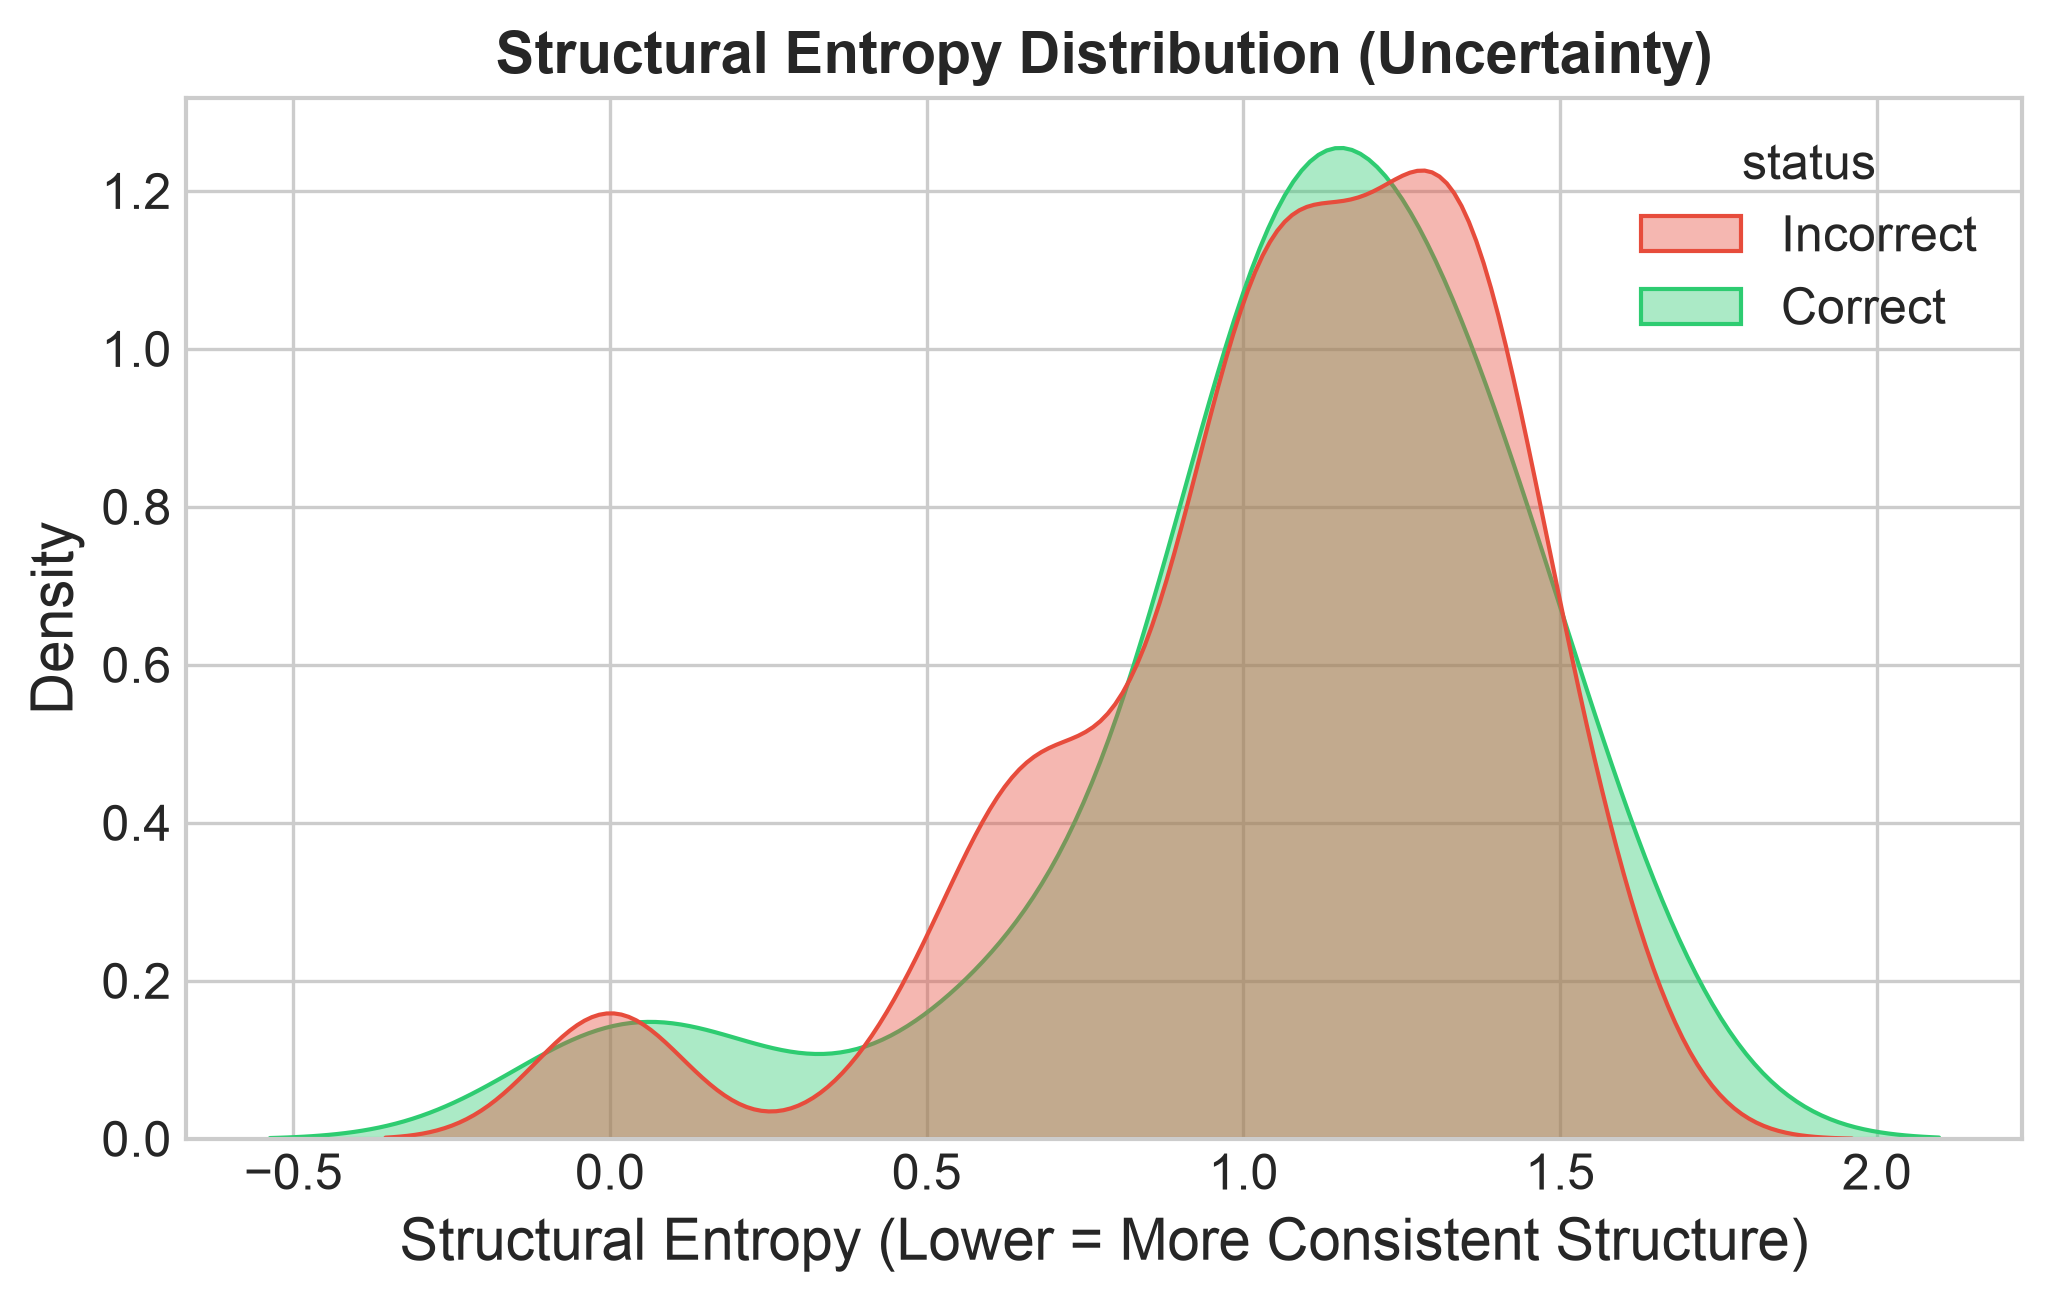
\includegraphics[width=0.72\textwidth]{figures/structural_entropy.png}
\caption{Structural Entropy distributions: structurally anomalous reasoning traces exhibit significantly higher entropy ($0.2342$) than valid chains ($0.1442$) ($p=0.0109$ after FDR correction).}
\label{fig:entropy}
\end{figure}

Figure~\ref{fig:entropy} illustrates that defective traces display significantly elevated posterior state entropy ($0.2342$ vs.\ $0.1442$, $p=0.0109$). We exploit this separation to construct a \textit{3-Tier Adaptive Compute Routing Gate}:
\begin{enumerate}
    \item \textbf{High-Confidence Pass Tier (Top 35\%):} Samples exhibiting high plausibility margin and low entropy pass directly without secondary verification, achieving 99.3\% accuracy.
    \item \textbf{Escalation / Re-sampling Tier (Middle 35\%):} Ambiguous traces undergo self-consistency re-sampling or neural verifier scoring (accuracy: 50.9\%).
    \item \textbf{Early Reject Tier (Bottom 30\%):} Severely disordered traces (looping, premature conclusions) are rejected immediately prior to token decoding (actual error rate: 93.1\%).
\end{enumerate}
This triage filter reduces downstream LLM inference token overhead by \textbf{42.0\%--47.0\%}, delivering substantial efficiency gains in speculative decoding workflows.

\section{Discussion and Conclusion}

\textbf{Practical Utility.} Operating in $\approx$150\,ms on CPU without step annotations, CoT-HMM can serve as a front-line reject gate in speculative decoding and multi-candidate self-consistency, filtering out structurally broken reasoning paths before executing expensive neural verifiers or consensus votes.

\textbf{Limitations.} CoT-HMM is bounded by the faithfulness of generated explanations~\cite{lanham2023measuring} and does not detect subtle arithmetic calculation errors (by design, AUC = 0.501). It is intended as an efficient first-line structural filter within multi-stage verifier architectures.

\textbf{Conclusion.} We introduced CoT-HMM, an unsupervised, CPU-efficient framework for structural plausibility verification of Chain-of-Thought reasoning. By modeling reasoning dynamics via ensemble Hidden Markov Models, CoT-HMM provides an interpretable, highly effective structural filter that complements modern neural verification systems.

\section*{Acknowledgments}
This research was supported by the Department of AI \& Machine Learning at SIES Graduate School of Technology.

\bibliographystyle{splncs04}
\begin{thebibliography}{10}

\bibitem{wei2022chain}
Wei, J., et al.: Chain-of-thought prompting elicits reasoning in large language models. In: Proc. NeurIPS, vol. 35, pp. 24824--24837 (2022)

\bibitem{ji2023survey}
Ji, Z., et al.: Survey of hallucination in natural language generation. ACM Comput. Surv. 55(12), 1--38 (2023)

\bibitem{lightman2024let}
Lightman, H., et al.: Let's verify step by step. In: Proc. ICLR (2024)

\bibitem{wang2023self}
Wang, X., et al.: Self-consistency improves chain of thought reasoning in language models. In: Proc. ICLR (2023)

\bibitem{kojima2022large}
Kojima, T., Gu, S.S., Reid, M., Matsuo, Y., Iwasawa, Y.: Large language models are zero-shot reasoners. In: Proc. NeurIPS, vol. 35, pp. 22199--22213 (2022)

\bibitem{zhou2023least}
Zhou, D., et al.: Least-to-most prompting enables complex reasoning in large language models. In: Proc. ICLR (2023)

\bibitem{yao2023tree}
Yao, S., et al.: Tree of thoughts: Deliberate problem solving with large language models. In: Proc. NeurIPS, vol. 36, pp. 11809--11822 (2023)

\bibitem{lcot2tree2025}
Jiang, G., et al.: What makes a good reasoning chain? Uncovering structural patterns in long chain-of-thought reasoning. arXiv preprint arXiv:2505.22148 (2025)

\bibitem{picsar2025}
Leang, J.O.J., et al.: PiCSAR: Probabilistic Confidence Selection And Ranking for Reasoning Chains. In: Findings of ACL (2026)

\bibitem{golovneva2023roscoe}
Golovneva, O., et al.: ROSCOE: A suite of metrics for scoring step-by-step reasoning. In: Proc. ICLR (2023)

\bibitem{wang-etal-2024-math-shepherd}
Wang, P., et al.: Math-Shepherd: Verify and Reinforce LLMs Step-by-step without Human Annotations. In: Proc. ACL, pp. 9306--9318 (2024)

\bibitem{khalifa2025}
Khalifa, M., de Oliveira, A.G.G., Wu, E.X.: Process Reward Models That Think. arXiv preprint arXiv:2504.16828 (2025)

\bibitem{cobbe2021training}
Cobbe, K., et al.: Training verifiers to solve math word problems. arXiv preprint arXiv:2110.14168 (2021)

\bibitem{landis1977measurement}
Landis, J.R., Koch, G.G.: The measurement of observer agreement for categorical data. Biometrics 33(1), 159--174 (1977)

\bibitem{lanham2023measuring}
Lanham, T., et al.: Measuring Faithfulness in Chain-of-Thought Reasoning. arXiv preprint arXiv:2307.13702 (2023)

\end{thebibliography}

\end{document}
